\documentclass[a4paper,11pt]{report}
\usepackage[T1]{fontenc}
\usepackage[utf8]{inputenc}
\usepackage{lmodern}
\usepackage{graphicx}
\usepackage{listings}
\usepackage[margin=1in]{geometry}
\usepackage[hidelinks]{hyperref}

\title{Telnet Control of a VLC Daemon}
\author{Darryn Anton Jordan \\\href{mailto:jrddar001@myuct.ac.za}{jrddar001@myuct.ac.za}}

\begin{document}

\maketitle
\tableofcontents

\lstdefinestyle{customc}{
  belowcaptionskip=1\baselineskip,
  breaklines=true,
  frame=L,
  xleftmargin=\parindent,
  language=C++,
  showstringspaces=false,
  basicstyle=\footnotesize\ttfamily,
}

\newpage

\section{Introduction}
This document details the method used to initiate and terminate recordings of a live feed, streamed from an IP camera using VLC (VideoLAN Client) in telnet interface.\\\\
In order to avoid confusion, some terms will now be introduced. Each radar node will be referred to as a server. This server will run VLC in its daemon mode and have a network connection to the IP camera.\\
The computer used to control and make requests from the server will be referred to as a client.

\subsection{Software and Hardware Used}
\begin{itemize}
  \item Ubuntu 15.04
  \item VLC 2.2.0 Weatherwax
  \item Code::Blocks 13.12
  \item Boost Asio Library
  \item Wireshark 1.12.1 
  \item AVTECH AVM565A IP Camera
\end{itemize}

\newpage

\section{Preparation and Set-up}
\subsection{Server}
The server is required to have VLC installed (easily found in the Ubuntu Software Centre). Once installed, a password and host for telnet connections must be set. This can be found by navigating to Tools>Preferences>Show All Settings>Interface>Main Interfaces>Lua.
\begin{figure}[h]
  \begin{center}
    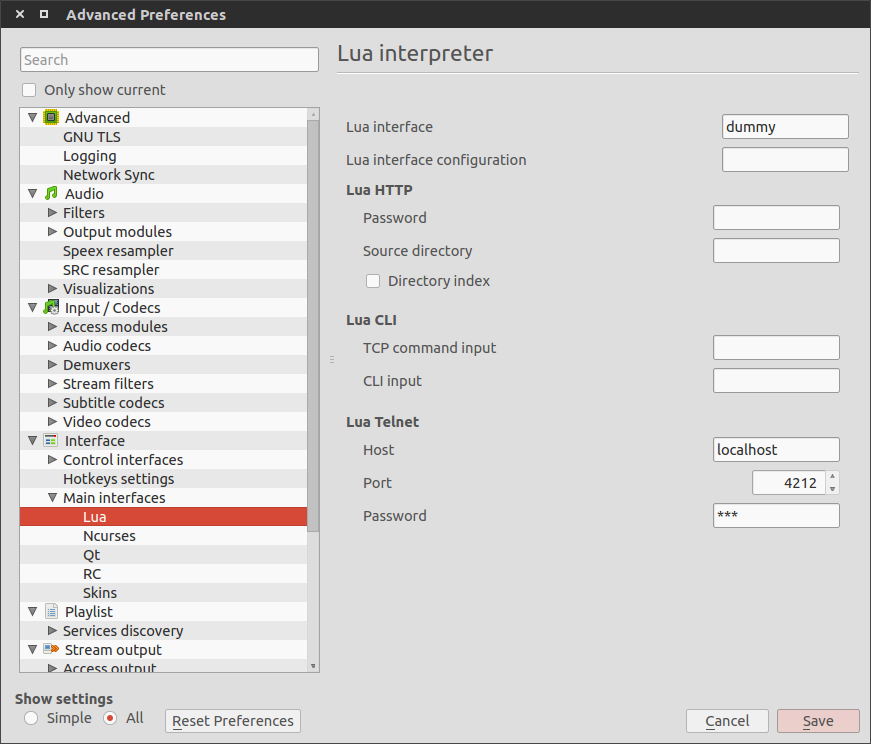
\includegraphics[scale = 0.4]{settings}
    \caption{Telnet Settings}
  \end{center}
\end{figure} \\
As seen in the figure above, the host is set to 'localhost' (or 127.0.0.1), the default port is '4212' and the password is set to 'vlc' for simplicity. In order to launch VLC in its daemon telnet interface, the following command is run in terminal.
\begin{lstlisting}
vlc -I telnet
\end{lstlisting}
If the response shown in the figure below is returned, then the server is ready to be controlled.   
\begin{figure}[h]
   \begin{center}
     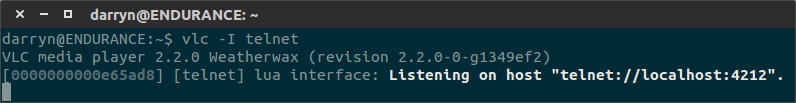
\includegraphics[scale=0.5]{server_vlc}
     \caption{VLC Telnet Server}
   \end{center}
 \end{figure} \\ 
We now require the IP address of the network camera connected to the server. See Appendix A for one way of finding this. 

\subsection{Software Development}
Code::Blocks and the Asio Boost Library were used to develop the C++ application responsible for socket communication to the VLC daemon.

\subsubsection{Prerequisites}
The following terminal commands will ensure all prerequisites for development (g++ compiler and Boost) are present. 
\begin{lstlisting}
sudo apt-get install build-essential
sudo apt-get install libboost-all-dev
\end{lstlisting}
The project can now be opened in Code::Blocks, but \textbf{must} be cleaned and rebuilt.

\subsubsection{Expected Results}
After compiling the program, the user is presented with the following console.
\begin{figure}[h]
   \begin{center}
     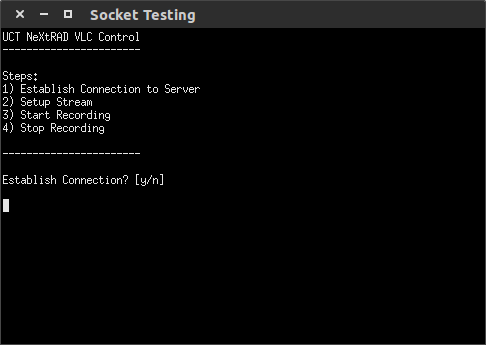
\includegraphics[scale=0.5]{Console_1}
     \caption{VLC Socket Controller Welcome}
   \end{center}
 \end{figure} \\
If the server is configured correctly, then the following response is returned. The program is now connected and a stream can be established.
 \begin{figure}[h]
   \begin{center}
     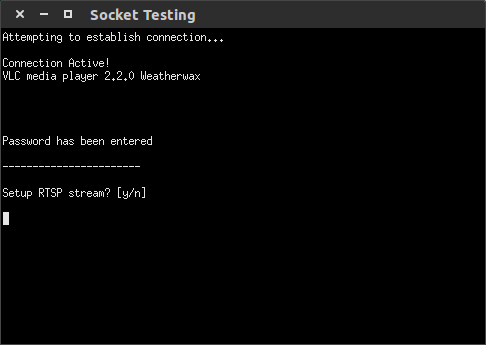
\includegraphics[scale=0.5]{Console_2}
     \caption{Connection Established}
   \end{center}
 \end{figure} \\
The following figure shows that the program displays all commands to be sent to the VLC daemon. Parameters such as the IP address, port number and path to overlay image and must obviously be modified. 
 \begin{figure}[h]
   \begin{center}
     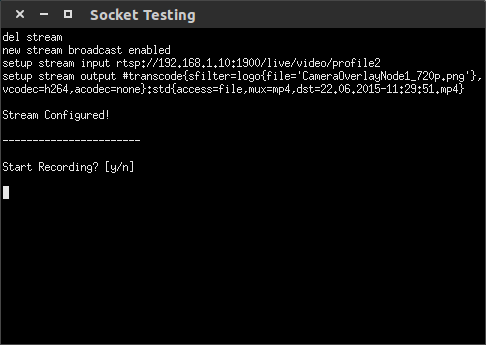
\includegraphics[scale=0.5]{Console_3}
     \caption{Stream Settings}
   \end{center}
 \end{figure} \\ 
Once the stream is terminated, the program produces a .mpg file in the home directory with the computers date and time as its filename. Below is a screenshot of a sample output.
 \begin{figure}[h]
   \begin{center}
     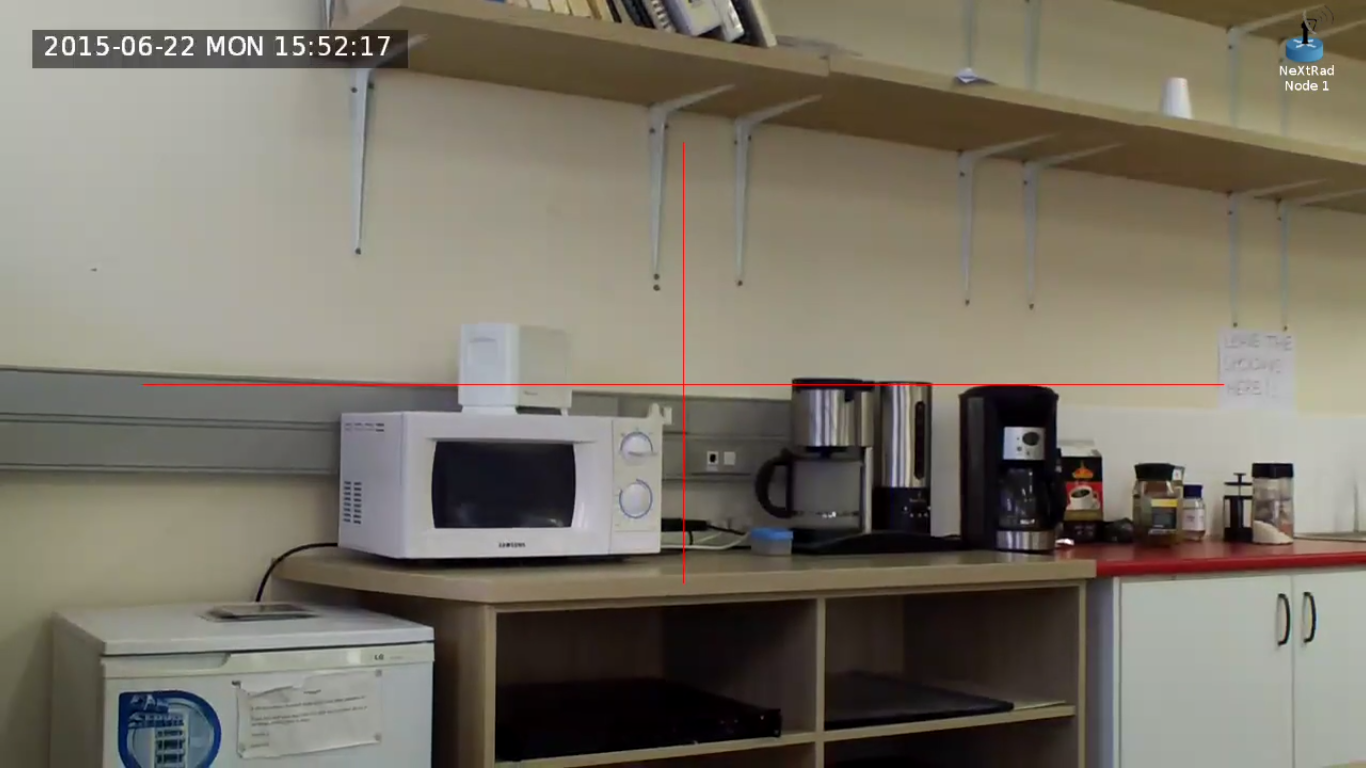
\includegraphics[scale=0.3]{demo}
     \caption{Example Output}
   \end{center}
 \end{figure} \\
Note: in this test, Profile 2 was used (1280x720). The correspondingly sized image overlay (CameraOverlayNode1\_720p) had to be used.

\subsubsection{Possible Source of Confusion}
Please note that if the camera has been reset, and the default settings are active, then the camera does not allow for anonomous login. This means that in order to access a RTSP stream, the admin username and password must be entered. In this case, \textbf{no video will be recorded}. The program cannot account for this. Please refer to the following section, for a guide on activating anonomous login.

\section{Camera Streaming Settings}
Once the network camera's IP address is known, various settings can be tweaked. Opening \url{http://camera_ip_address:port_number} allows an admin to alter these settings. By default the username and password are \textit{admin}.
 \begin{figure}[h]
   \begin{center}
     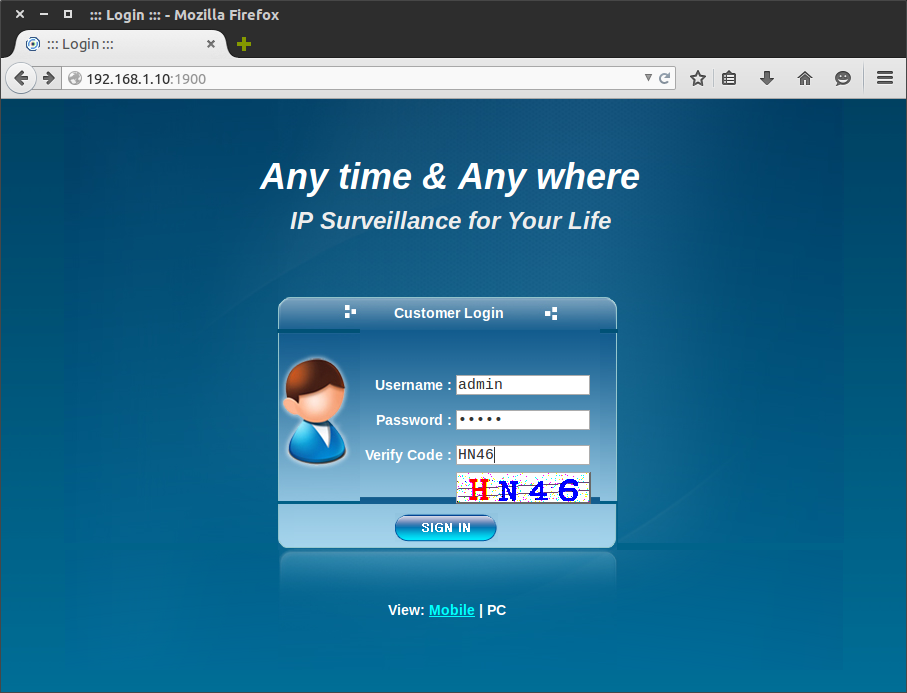
\includegraphics[scale=0.3]{camera_login}
     \caption{Camera Login}
   \end{center}
 \end{figure}
\subsubsection{Video Profiles}
Navigating to Config>Camera>Video allows the admin to configure the streaming profiles. During development it was decided that Profile 2 would be used for 1280x720 recording and that Profile 3 would possibly be a lower resolution for live streaming to the client. 
 \begin{figure}[h]
   \begin{center}
     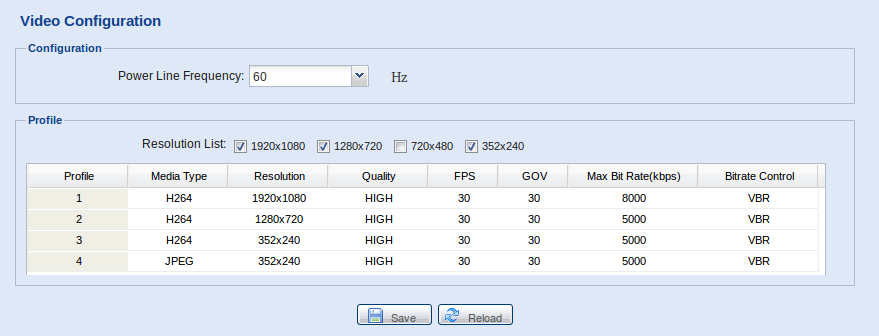
\includegraphics[scale=0.4]{video_config}
     \caption{Profile Configuration}
   \end{center}
 \end{figure} \\
These profiles can be individually tested using VLC. Each stream is accessable at\\ \url{rtsp://camera_ip_address:port_number/live/video/profile(1/2/3/4)}\\\\ e.g. \url{rtsp://192.168.1.10:1900/live/video/profile2}
\subsubsection{Anonomous Login}
It is \textbf{vital} that anonomous login be enabled for video recording to be possible. Navigate to Config>General>Online and ENABLE anonomous login. This is automatically set to disabled upon camera reset.
 \begin{figure}[h]
   \begin{center}
     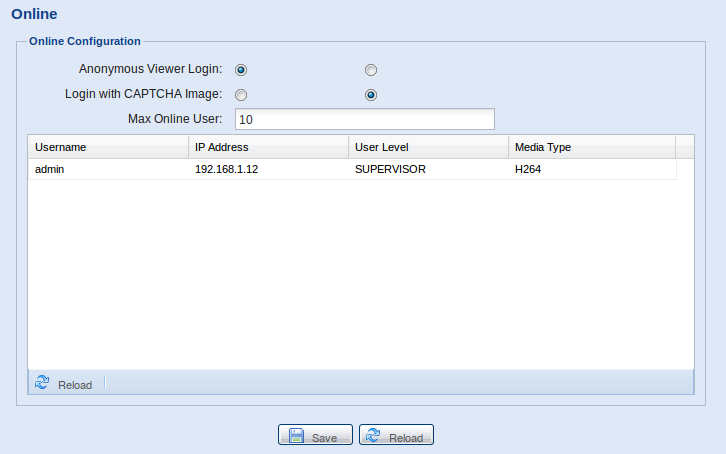
\includegraphics[scale=0.4]{online}
     \caption{Online Configuration}
   \end{center}
 \end{figure}

\section{Addtitional Information}
\begin{itemize}
  \item Basics of the VLC telnet interface: \\ \url{http://www.videolan.org/doc/streaming-howto/en/ch05.html}
  \item VLC Streaming options: \\ \url{http://www.videolan.org/doc/streaming-howto/en/ch03.html}
\end{itemize}

\newpage
\section*{Appendix A: Finding the IP Address of an AVTECH Network Camera} 
\begin{itemize}
  \item Supply the camera with power (12V, 1A).
  \item Connect to camera using Ethernet cable.
  \item Set computer IP address to 192.168.1.1
  \item Install Wireshark, with some additional tweaking:
\begin{lstlisting}
sudo chgrp myusername /usr/bin/dumpcap
sudo chmod 750 /usr/bin/dumpcap
sudo setcap cap_net_raw,cap_net_admin+eip /usr/bin/dumpcap
\end{lstlisting}
\item Monitor the connections with IP Cam over the Ethernet connection. The IP can be found in an AVTECH broadcast. In this example; 192.168.1.10. 
 \begin{figure}[h]
   \begin{center}
     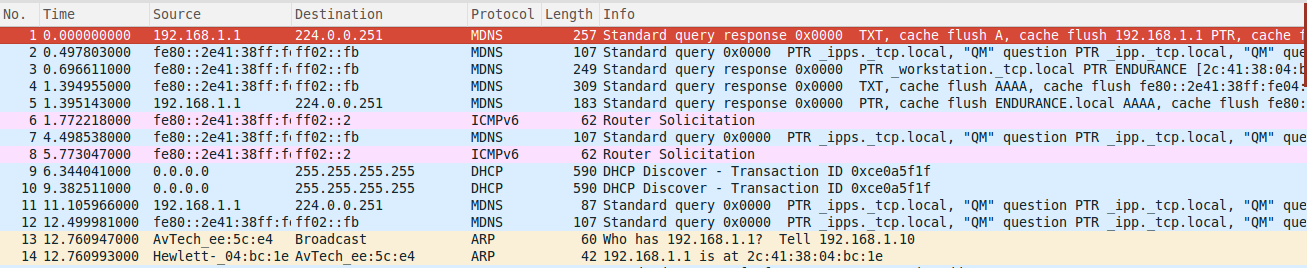
\includegraphics[scale=0.34]{IP}
   \end{center}
 \end{figure}
\item Open web browser: http://192.168.1.10:1900. Default username (admin) and password (admin).
\item (Optional) for live viewing in the browser, install:
\begin{lstlisting}
sudo apt-get install vlc browser-plugin-vlc
\end{lstlisting}

\end{itemize}

\begin{figure}[h]
 \begin{center}
   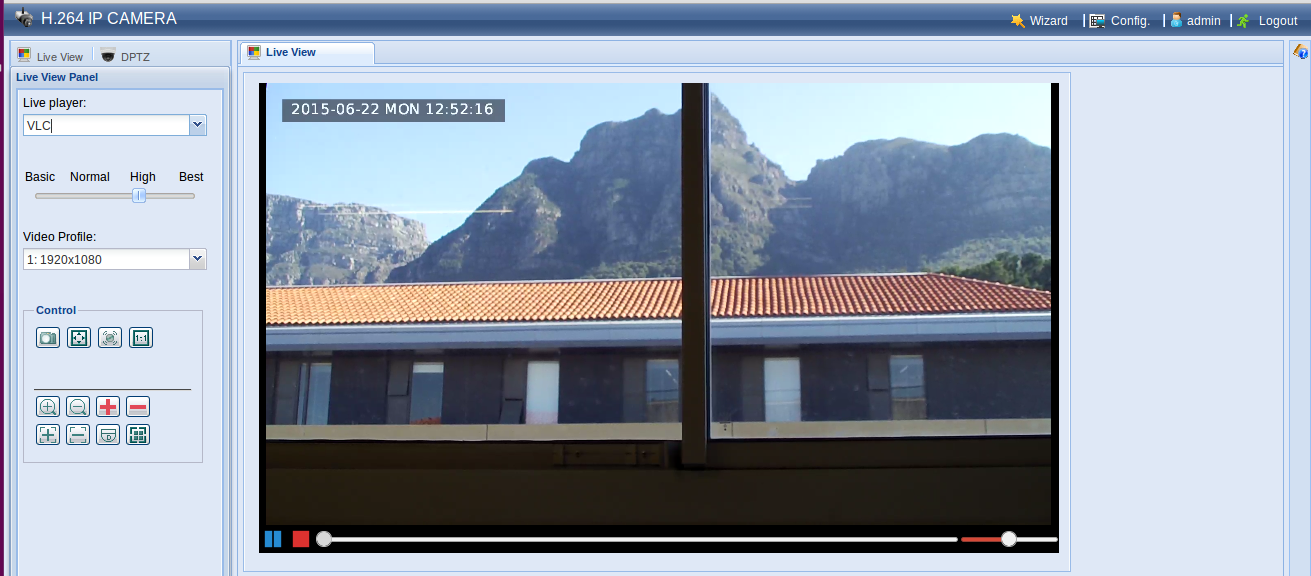
\includegraphics[scale=0.34]{live}
 \end{center}
\end{figure}

\newpage
\section*{Appendix B: Code Listing}

\lstset{escapechar=@,style=customc}
\lstinputlisting[style=customc]{main.cpp}



\end{document}
